\documentclass[journal, onecolumn, 12pt]{IEEEtran}

\usepackage{hyperref}
\usepackage[utf8]{inputenc}
\usepackage{graphicx}
\usepackage{color}
\usepackage{listings}

\graphicspath{{figures/}}

\definecolor{dkgreen}{rgb}{0,0.6,0}
\definecolor{gray}{rgb}{0.5,0.5,0.5}
\definecolor{mauve}{rgb}{0.58,0,0.82}

\lstset{frame=tb,
  language=C,
  aboveskip=3mm,
  belowskip=3mm,
  showstringspaces=false,
  columns=flexible,
  basicstyle={\small\ttfamily},
  numbers=none,
  numberstyle=\tiny\color{gray},
  keywordstyle=\color{blue},
  commentstyle=\color{dkgreen},
  stringstyle=\color{mauve},
  breaklines=true,
  breakatwhitespace=true,
  tabsize=4
}

\hypersetup{
    colorlinks=true,
    linkcolor=blue,
    filecolor=blue,
    urlcolor=blue,
    citecolor=cyan,
}

%opening
\title{Journal of A Simple Compiler}
\author{Trganda}

\begin{document}

\maketitle

\section{Part 0: Introduction}

I've decided to go on a compiler writing journey.
In the past I've written some \href{https://github.com/DoctorWkt/pdp7-unix/blob/master/tools/as7}{assemblers},
and I've written a \href{https://github.com/DoctorWkt/h-compiler}{simple compiler} for a typeless language.
But I've never written a compiler that can compile itself.
So that's where I'm headed on this journey.

As part of the process, I'm going to write up my work so that others can follow along.
This will also help me to clarify my thoughts and ideas. Hopefully you, and I, will find this useful!s

\subsection{Goals of the journey}

Here are my goals, and non-goals, for the journey:

\begin{itemize}
    \item To write a self-compiling compiler. I think that if the compiler can compile itself, it gets to call itself a real compiler.
    \item To target at least one real hardware platform. I've seen a few compilers that generate code for hypothetical machines.
          I want my compiler to work on real hardware. Also, if possible, I want to write the compiler so that it can support multiple backends for different hardware platforms.
    \item Practical before research. There's a whole lot of research in the area of compilers. I want to start from absolute zero on this journey, so I'll tend to go for a practical approach and not a theory-heavy approach. That said, there will be times when I'll need to introduce (and implement) some theory-based stuff.
    \item Follow the KISS principle: keep it simple, stupid! I'm definitely going to be using Ken Thompson's Principe here: "When in doubt, use brute force."
    \item Take a lot of small steps to reach the final goal. I'll break the journey up into a lot of simple steps instead of taking large leaps. This will make each new addition to the compiler a bite-sized and easily digestible thing.
\end{itemize}

\subsection{Target Language}

The choice of a target language is diffcult. If I choose a high-level language like \textbf{Python}, \textbf{Go} etc., then I'll have to implement a whole pile of libraries and classes as they are built-in to the language.

I could write a compiler for a language like Lisp, but these can be \href{ftp://publications.ai.mit.edu/ai-publications/pdf/AIM-039.pdf}{done easily}.

Instead, I've fallen back on the old standby and I'm going to write a compiler for a subset of C, enough to allow the compiler to compile itself. C is just a step up from assembly language (for some subset of C, not \href{https://en.wikipedia.org/wiki/C18_(C_standard_revision)}{C18}), and this will help make the task of compiling the C code down to assembly somewhat easier. Oh, and I also like C.

\subsection{The Basic of a Compiler's Job}

The job of a compiler is to translate input in one language (usually a high-level language) into a different output language (usually a lower-level language than the input). The main steps are:

\begin{figure}[!ht]
    \centering
    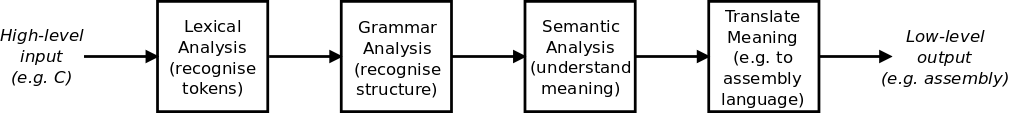
\includegraphics[width= 0.9\textwidth]{parsing_steps.png}
\end{figure}

\begin{itemize}
    \item Do \href{https://en.wikipedia.org/wiki/Lexical_analysis}{lexical analysis} to recognize the lexical elements. In several languages, {\color{red}=} is different to {\color{red}==}, so you can't just read a single {\color{red}=}. We call these lexical elements \textit{tokens}.
    \item \href{https://en.wikipedia.org/wiki/Parsing}{Parse} the input, i.e. recognize the syntax and structural elements of the input and ensure that they conform to the \textit{grammar} of the language. For example, your language might have this decision-making structure:
    \begin{lstlisting}
if (x < 23) {
    print("x is smaller than 23\n");
}
    \end{lstlisting}
    but in another language you might write:
    \begin{lstlisting}
if (x < 23)
    print("x is smaller than 23\n");
    \end{lstlisting}
    This is also the place where the compiler can detect syntax errors, like if the semicolon was missing on the end of first \textit{print} statement.
    \item Do \href{https://en.wikipedia.org/wiki/Semantic_analysis_(compilers)}{semantic analysis} of the input, i.e. understand the meaning of the input. This is actually different from recognising the syntax and structure. For example, in English, a sentence might have the form \textbf{<subject> <verb> <adjective> <object>}.
    \begin{lstlisting}
David ate lovely bananas.
Jennifer hates green tomatoes.
    \end{lstlisting}
    \item \href{https://en.wikipedia.org/wiki/Code_generation_(compiler)}{Translate} the meaning of the input into a different language. Here we convert the input, parts at a time, into a lower-level language.
\end{itemize}

\subsection{Resources}

There's a lot of compiler resources out on the Internet. Here are the ones I'll be looking at.

\subsubsection{Learning Resources}

If you want to start with some books, papers and tools on compilers, I'd highly recommend this list:

\begin{itemize}
    \item \href{https://github.com/aalhour/awesome-compilers}{Curated list of awesome resources on Compilers, Interpreters and Runtimes} by Ahmad Alhour
\end{itemize}

\subsubsection{Existing Compilers}

While I'm going to build my own compiler, I plan on looking at other compilers for ideas and probably also borrow some of their code. Here are the ones I'm looking at:

\begin{itemize}
    \item \href{http://www.t3x.org/subc/}{SubC} by Nils M Holm
    \item \href{https://github.com/rswier/swieros/blob/master/root/bin/c.c}{Swieros C Compiler} by Robert Swierczek
    \item \href{https://github.com/DoctorWkt/fbcc}{fbcc} by Fabrice Bellard
    \item \href{https://bellard.org/tcc}{tcc}, also by Fabrice Bellard and others
    \item \href{https://github.com/yui0/catc}{catc}  by Yuichiro Nakada
    \item \href{https://github.com/jserv/amacc}{amacc} by Jim Huang
    \item \href{https://en.wikipedia.org/wiki/Small-C}{Small C} by Ron Cain, James E. Hendrix, derivatives by others
\end{itemize}

In particular, I'll be using a lot of the ideas, and some of the code, from the SubC compiler.

\subsection{Setting Up the Development Environment}

Assuming that you want to come along on this journey, here's what you'll need. I'm going to use a Linux development environment, so download and set up your favorite Linux system: I'm using Lubuntu $18.04$.

I'm going to target two hardware platforms: Intel x86-64 and 32-bit ARM. I'll use a PC running Lubuntu $18.04$ as the Intel target, and a Raspberry Pi running Raspbian as the ARM target.

On the Intel platform, we are going to need an existing C compiler. So, install this package.
If there are any more tools required for a vanilla Linux system let me know.

Finally, clone a copy of this Github repository.

\subsection{The Next Step}

In the next part of our compiler writing journey, we will start with the code to scan our input file and find the \textit{tokens} that are the lexical elements of our language.

\section{Part 1: Introduction to Lexical Scanning}

We start our compiler writing journey with a simple lexical scanner. As I mentioned in the previous part, the job of the scanner is to identify the lexical elements, or \textit{tokens}, in the input language.

We will start with a language that has only five lexical elements:
\begin{itemize}
    \item the four basic maths operators: {+}, {/}, {+} and {-}
    \item decimal whole numbers which have 1 or more digits 0 .. 9
\end{itemize}

Each token that we scan is going to be stored in this structure (from \textbf{defs.h})

\begin{lstlisting}
// Token structure
struct token {
    int token;
    int intvalue;
};
\end{lstlisting}

where the \textbf{token} field can be one of these values (from \textbf{defs.h}):

\begin{lstlisting}
// Tokens
enum {
    T_PLUS, T_MINUS, T_STAR, T_SLASH, T_INTLIT
};
\end{lstlisting}

When the token is a $T\_INTLIT$ (i.e. an integer literal), the $intvalue$ field will hold the value of the integer that we scanned in.

\subsection{Functions in $scan.c$}

The $scan.c$ file holds the functions of our lexical scanner. We are going to read in one character at a time from our input file. However, there will be times when we need to "put back" a character if we have read too far ahead in the input stream. We also want to track what line we are currently on so that we can print the line number in our debug messages. All of this is done by the $next()$ function:

\begin{lstlisting}
    static int next(void) {
        int c;

        if (Putback) {                // Use the character put
            c = Putback;              // back if there is one
            Putback = 0;
            return c;
        }

        c = fgetc(Infile);            // Read from input file
        if ('\n' == c)
        Line++;                       // Increment line count
        return c;
    }
\end{lstlisting}

The $Putback$ and $Line$ variables are defined in $data.h$ along with our input file pointer:

\begin{lstlisting}
    extern_ int     Line;
    extern_ int     Putback;
    extern_ FILE    *Infile;
\end{lstlisting}

All C files will include this where $extern\_$ is replaced with $extern$. But $main.c$ will remove the $extern\_$; hence, these variables will "belong" to $main.c$.

Finally, how do we put a character back into the input stream? Thus:

\begin{lstlisting}
    // Put back an unwanted character
    static void putback(int c) {
        Putback = c;
    }
\end{lstlisting}

\subsection{Ignoring Whitespace}

We need a function that reads and silently skips whitespace characters until it gets a non-whitesapce character, and returns it. Thus:

\begin{lstlisting}
    // Skip past input that we don't nee   d to deal with,
    // i.e. whitesapce, newlines. Return the first
    // character we do need to deal with.
    static int skip(void) {
        int c;

        c = next();
        while (' ' == c || '\t' == c || '\n' == c || '\r' == c || '\f' == c) {
            c = next();
        }
        return (c);
    }
\end{lstlisting}

\subsection{Scanning Tokens: $scan()$}

So new we can read characters in while skipping whitespace; we can also put back a character if we read one character too far ahead. We can now write our first lexical scanner:

\begin{lstlisting}
    // Scan and return the next token found in the input.
    // Return 1 if token valid, 0 if no tokens left.
    int scan(struct token *t) {
      int c;

      // Skip whitespace
      c = skip();

      // Determine the token based on
      // the input character
      switch (c) {
      case EOF:
        return (0);
      case '+':
        t->token = T_PLUS;
        break;
      case '-':
        t->token = T_MINUS;
        break;
      case '*':
        t->token = T_STAR;
        break;
      case '/':
        t->token = T_SLASH;
        break;
      default:
        // More here soon
      }

      // We found a token
      return (1);
    }
\end{lstlisting}

That's it for the simple one-character tokens: for each recognized character, turn it into a token. You may ask: why not just put the recognized character into the $struct token$? The answer is that later we will need to recognized multi-character tokens such as $==$ and keywords like $if$ and $while$. So it will make life easier to have an enumerated list of token values.

\subsection{Integer Literal Values}

In fact, we already have to face this situation as we also need to recognize integer literal values like $3827$ and $87731$. Here is the missing $default$ code from the $switch$ statement:

\begin{lstlisting}
default:
    // If it's a digit, scan the
    // literal integer value in
    if (isdigit(c)) {
      t->intvalue = scanint(c);
      t->token = T_INTLIT;
      break;
    }

    printf("Unrecognised character %c on line %d\n", c, Line);
    exit(1);
\end{lstlisting}

Once we hit a decimal digit character, we call the helper function $scanint()$ with this first character. It will return the scanned integer value. To do this, it has to read each character in turn, check that it's a legitimate digit, and build up the final number. Here is the code:

\begin{lstlisting}
// Scan and return an integer literal
// value from the input file. Store
// the value as a string in Text.
static int scanint(int c) {
    int k, val = 0;

    // Convert each character into an int value
    while ((k = chrpos("0123456789", c)) >= 0) {
        val = val * 10 + k;
        c = next();
    }

    // We hit a non-integer character, put it back.
    putback(c);
    return val;
}
\end{lstlisting}

We start with a zero $val$ value. Each time we get a character in the set $0$ to $9$, we covert this to an $int$ value with $chrpos()$. We make $val$ 10 times bigger and then add this new digit to it.

For example, if we have the character $3$, $2$, $8$, we do:

\begin{itemize}
    \item $val = 0 * 10 + 3$, i.e. 3
    \item $val = 3 * 10 + 2$, i.e. 32
    \item $val = 32 * 10 + 8$, i.e. 328
\end{itemize}

Right at the end, did you notice the call to $putback(c)$? We found a character that's not a decimal digit at this point. We can't simply discard it, but luckily we can put it back in the input stream to be consumed later.

You may also ask at this point: why not simply substract the ASCII value of $0$ from $c$ to make it an integer? The answer is that, later on, we will be able to do $chrpos("0123456789abcdef")$ to convert hexadecimal digits as well.

Here's the code for $chrpos()$:

\begin{lstlisting}
    // Return the position of character c
    // in string s, or -1 if c not found
    static int chrpos(char *s, int c) {
      char *p;

      p = strchr(s, c);
      return (p ? p - s : -1);
    }
\end{lstlisting}

And that's it for the lexical scanner code in $scan.c$ for now.

\subsection{Putting the Scanner to Work}

The code in $main.c$ puts the above scanner to work. The $main()$ function opens up a file and then scans it for tokens:

\begin{lstlisting}
    void main(int argc, char *argv[]) {
        ...
        init();
        ...
        Infile = fopen(argv[1], "r");
        ...
        scanfile();
        exit(0);
    }
\end{lstlisting}

And $scanfile()$ loops while there is new token and prints out the details of the token:

\begin{lstlisting}
    // List of printable tokens
    char *tokstr[] = { "+", "-", "*", "/", "intlit" };

    // Loop scanning in all the tokens in the input file.
    // Print out details of each token found.
    static void scanfile() {
        struct token T;

        while (scan(&T)) {
            printf("Token %s", tokstr[T.token]);
            if (T.token == T_INTLIT)
                printf(", value %d", T.intvalue);
            printf("\n");
        }
    }
\end{lstlisting}

\subsection{Some Example Input Files}

I've provided some example input files so you can see what tokens the scanner finds in each file, and what input files the scanner rejects.

\begin{lstlisting}
    $ make
    cc -o scanner -g main.c scan.c

    $ cat input01
    2 + 3 * 5 - 8 / 3

    $ ./scanner input01
    Token intlit, value 2
    Token +
    Token intlit, value 3
    Token *
    Token intlit, value 5
    Token -
    Token intlit, value 8
    Token /
    Token intlit, value 3

    $ cat input04
    23 +
    18 -
    45.6 * 2
    / 18

    $ ./scanner input04
    Token intlit, value 23
    Token +
    Token intlit, value 18
    Token -
    Token intlit, value 45
    Unrecognised character . on line 3
\end{lstlisting}

\subsection{Conclusion and What's Next}

We've started small and we have a simple lexical scanner that recognizes the four main maths operators and also integer values. We saw that we needed to skip whitespace and put back characters if we read too far into the input.

Single character tokens are easy to scan, but multi-character tokens are a bit harder. But at the end, the $scan()$ function returns the next token from the input file in a $struct token$ variable.

In the next part of our compiler writing journey, we will build a recursive descent parser to interpret the grammar of our input files, and calculate \& print out the final value for each file.

\section{Part 2: Introduction to Parsing}

In this part of our compiler writing journey, I'm going to introduce the basics of a parser. As I mentioned in the first part, the job of the parser is to recognize the syntax and structural elements of the input and ensure that they conform to the $grammer$ of the language.

We already have several language elements that we can scan in, i.e. our tokens:

\begin{itemize}
    \item the four basic maths operators: $*, /, +$ and $-$
    \item deciaml whole numbers which have $1$ or more digits $0$ .. $9$
\end{itemize}

Now let's define a grammar for the language that our parser will recognize.

\subsection{BNF: Backus-Naur Form}

You will come across the use of \href{https://en.wikipedia.org/wiki/Backus%E2%80%93Naur_form}{BNF} at some point if you get into dealing with computer languages. I will just introduce enough of the BNF syntax here to express the grammar we want to recognize.

We want a grammar to express maths expressions with whole numbers. Here is the BNF description of the grammar:

\begin{lstlisting}
    expression: number
    | expression '*' expression
    | expression '/' expression
    | expression '+' expression
    | expression '-' expression
    ;

    number:  T_INTLIT
    ;
\end{lstlisting}

The vertical bars separate options in the grammar, so the above says:

\begin{itemize}
    \item An expression could be just a number, or
    \item An expression is two expressions separated by a $*$ token, or
    \item An expression is two expressions separated by a $/$ token, or
    \item An expression is two expressions separated by a $+$ token, or
    \item An expression is two expressions separated by a $-$ token, or
    \item A number is always a $T\_INTLIT$ token
\end{itemize}

It should be pretty obvious that the BNF definition of the grammar is $recursive$: an expression is defined by referencing other expressions. But there is a way to \textbf{bottom-out} the recursion: when an expression turns out to be a number, this is always a $T\_INTLIT$ token and thus not recursive.

In BNF, we say that "expression" and "number" are $non-termainl$ symbols, as they are produced by rules in the grammar. However, $T\_INTLIT$ is a $terminal$ symbol as it is not defined by any rule. Instead, it is an already-recognized token in the language. Similarly, the four maths operator tokens are terminal symbols.

\subsection{Recursive Descent Parsing}

Given that the grammar for our language is recursive, it makes sense for us to try and parse it recursively. What we need to do is to read in a token, then $look ahead$ to the next token. Based on what the next token is, we can then decide what path we need to take to parse the input. This may require us to recursively call a function that has already been called.

In our case, the first token in any expression will be a number and this may be followed by maths operator. After that there may only be a single number, or there may be the start of a whole new expression. How can we parse this recursively?

We can write pseudo-code that look like this:

\begin{lstlisting}
    function expression() {
        Scan and check the first token is a number. Error if it's not
        Get the next token
        If we have reached the end of the input, return, i.e. base case

        Otherwise, call expression()
    }
\end{lstlisting}

Let's run this function on the input $2 + 3 - 5\quad T\_EOF$ where $T\_EOF$ is a token that reflects the end of the input. I will number each call to $expression()$.

\begin{lstlisting}
    expression0:
    Scan in the 2, it's a number
    Get next token, +, which isn't T_EOF
    Call expression()

      expression1:
        Scan in the 3, it's a number
        Get next token, -, which isn't T_EOF
        Call expression()

          expression2:
            Scan in the 5, it's a number
            Get next token, T_EOF, so return from expression2

        return from expression1
    return from expression0
\end{lstlisting}

Yes, the function was able to recursively parse the input $2 + 3 - 5\quad T\_EOF$.

Of course, we haven't done anything with the input, but that isn't the job of the parser. The parser's job is to $recognise$ the input, and warn of any syntax errors. Someone else is going to do the $semantic analysis$ of the input, i.e. to understand and perform the meaning of this input.

\begin{quote}
Later on, you will see that this isn't actually true. It often makes sense to intertwine the syntax analysis and semantic analysis.
\end{quote}

\subsection{Abstract Syntax Trees}

To do the semantic analysis, we need code that either interprets the recoginsed input, or translates it to another format, e.g. assembly code. In this part of the journey, we will build an interpreter for the input. But to get there, we are first going to convert the input into an \href{https://en.wikipedia.org/wiki/Abstract_syntax_tree}{abstract syntax tree} also known as an AST.

I highly recommend you read this short explanation of ASTs:
\begin{itemize}
    \item \href{https://medium.com/basecs/leveling-up-ones-parsing-game-with-asts-d7a6fc2400ff}{Leveling Up One’s Parsing Game With ASTs} by Vaidehi Joshi
\end{itemize}

It's well written and really help to explain the purpose and structure of ASTs. Don't worry, I'll be here when you get back.

The structure of each node in the AST that we will build is described in $defs.h$:

\begin{lstlisting}
    // AST node types
    enum {
      A_ADD, A_SUBTRACT, A_MULTIPLY, A_DIVIDE, A_INTLIT
    };

    // Abstract Syntax Tree structure
    struct ASTnode {
      int op;                               // "Operation" to be performed on this tree
      struct ASTnode *left;                 // Left and right child trees
      struct ASTnode *right;
      int intvalue;                         // For A_INTLIT, the integer value
    };
\end{lstlisting}

Some AST nodes, like those with $op$ values A\_ADD and A\_SUBTRACT have two child ASTs that are pointed to by $left$ and $right$. Later on, we will add or subtract the values of the sub-trees.

Alternatively, an AST node with the $op$ value A\_INTLIT represents an integer value. It has no sub-tree children, just a value in the $intvalue$ field.

\subsection{Building AST Nodes and Trees}

The code in $tree.c$ has the functions to build ASTs. The most general function, $mkastnode()$ takes values for all four fields in an AST node. It allocates the node, populates the field values and returns a pointer to the node:

\begin{lstlisting}
    // Build and return a generic AST node
    struct ASTnode *mkastnode(int op, struct ASTnode *left,
                              struct ASTnode *right, int intvalue) {
      struct ASTnode *n;

      // Malloc a new ASTnode
      n = (struct ASTnode *) malloc(sizeof(struct ASTnode));
      if (n == NULL) {
        fprintf(stderr, "Unable to malloc in mkastnode()\n");
        exit(1);
      }
      // Copy in the field values and return it
      n->op = op;
      n->left = left;
      n->right = right;
      n->intvalue = intvalue;
      return (n);
    }
\end{lstlisting}

Given this, we can write more specific functions that make a leaf AST node (i.e. one with no children), and make an AST node with a single child:

\begin{lstlisting}
    // Make an AST leaf node
    struct ASTnode *mkastleaf(int op, int intvalue) {
      return (mkastnode(op, NULL, NULL, intvalue));
    }

    // Make a unary AST node: only one child
    struct ASTnode *mkastunary(int op, struct ASTnode *left, int intvalue) {
      return (mkastnode(op, left, NULL, intvalue));
    }
\end{lstlisting}

\subsection{Purpose of the AST}

We are going to use an AST to store each expression that we recognise so that, later on, we can traverse it recursively to calculate the final value of the expression. We do want to deal with the precedence of the maths operators. Here is an example.

Consider the expression $2*3+4*5$. Now, multiplication has higher precedence that addition. Therefore, we want to $bind$ the multiplication operands together and perform these operations before we do the addition.

If we generated the AST tree to look like this:

\begin{lstlisting}
      +
     / \
    /   \
   /     \
  *       *
 / \     / \
2   3   4   5
\end{lstlisting}

then, when traversing the tree, we would perform $2*3$ first, then $4*5$. Once we have these results, we can then pass them up to the root of the tree to perform the addition.

\subsection{A Naive Expression Parser}

Now, we could re-use the token values from our scanner as the AST node operation values, but I like to keep the concept of tokens and AST nodes separate. So, to start with, I'm going to have a function to map the token values into AST node operation values. This, along with the rest of the parser, is in $expr.c$:

\begin{lstlisting}
    // Convert a token into an AST operation.
    int arithop(int tok) {
      switch (tok) {
        case T_PLUS:
          return (A_ADD);
        case T_MINUS:
          return (A_SUBTRACT);
        case T_STAR:
          return (A_MULTIPLY);
        case T_SLASH:
          return (A_DIVIDE);
        default:
          fprintf(stderr, "unknown token in arithop() on line %d\n", Line);
          exit(1);
      }
    }
\end{lstlisting}

The default statement in the switch statement fires when we can't convert the given token into an AST node type. It's going to form part of the syntax checking in our parser.

We need a function to check that the next token is an integer literal, and to build an AST node to hold the literal value. Here it is:

\begin{lstlisting}
    // Parse a primary factor and return an
    // AST node representing it.
    static struct ASTnode *primary(void) {
      struct ASTnode *n;

      // For an INTLIT token, make a leaf AST node for it
      // and scan in the next token. Otherwise, a syntax error
      // for any other token type.
      switch (Token.token) {
        case T_INTLIT:
          n = mkastleaf(A_INTLIT, Token.intvalue);
          scan(&Token);
          return (n);
        default:
          fprintf(stderr, "syntax error on line %d\n", Line);
          exit(1);
      }
    }
\end{lstlisting}

This assumes that there is a global variable $Token$, and that it already has the most recent token scanned in from the input. In $data.h$:

\begin{lstlisting}
    extern_ struct token    Token;
\end{lstlisting}

and in $main()$:

\begin{lstlisting}
    scan(&Token);                 // Get the first token from the input
    n = binexpr();                // Parse the expression in the file
\end{lstlisting}

Now we can write the code for the parser:

\begin{lstlisting}
    // Return an AST tree whose root is a binary operator
    struct ASTnode *binexpr(void) {
      struct ASTnode *n, *left, *right;
      int nodetype;

      // Get the integer literal on the left.
      // Fetch the next token at the same time.
      left = primary();

      // If no tokens left, return just the left node
      if (Token.token == T_EOF)
        return (left);

      // Convert the token into a node type
      nodetype = arithop(Token.token);

      // Get the next token in
      scan(&Token);

      // Recursively get the right-hand tree
      right = binexpr();

      // Now build a tree with both sub-trees
      n = mkastnode(nodetype, left, right, 0);
      return (n);
    }
\end{lstlisting}

Notice that nowhere in this naive parser code is there anything to deal with different operator precedence. As it stands, the code treats all operators as having equal precedence. If you follow the code as it parser the expression $2*3+4*5$, you will see that it builds this AST:

\begin{lstlisting}
     *
    / \
   2   +
      / \
     3   *
        / \
       4   5
\end{lstlisting}

This is definitely not correct. It will multiply $4*5$ to get 20, then do $3+20$ to ge $23$ insetad of doing $2*3$ to get 6.

So why did I do this? I wanted to show you that writign a simple parser is easy, but getting it to also do the semantic analysis is harder.

\subsection{Interpreting the Tree}

Now that we have our (incorrect) AST tree, let's write some code to interpret it. Again, we are going to write recursive code to traverse the tree. Here's the pseudo-code:

\begin{lstlisting}
    interpretTree:
    First, interpret the left-hand sub-tree and get its value
    Then, interpret the right-hand sub-tree and get its value
    Perform the operation in the node at the root of our tree
    on the two sub-tree values, and return this value
\end{lstlisting}

Going back to the correct AST tree:

\begin{lstlisting}
          +
         / \
        /   \
       /     \
      *       *
     / \     / \
    2   3   4   5
\end{lstlisting}

the call structure would look like:

\begin{lstlisting}
    interpretTree0(tree with +):
    Call interpretTree1(left tree with *):
       Call interpretTree2(tree with 2):
         No maths operation, just return 2
       Call interpretTree3(tree with 3):
         No maths operation, just return 3
       Perform 2 * 3, return 6

    Call interpretTree1(right tree with *):
       Call interpretTree2(tree with 4):
         No maths operation, just return 4
       Call interpretTree3(tree with 5):
         No maths operation, just return 5
       Perform 4 * 5, return 20

    Perform 6 + 20, return 26
\end{lstlisting}

\subsection{Code to Interpret the Tree}

This is in $interp.c$ and follows the above pseudo-code:

\begin{lstlisting}
    // Given an AST, interpret the
    // operators in it and return
    // a final value.
    int interpretAST(struct ASTnode *n) {
      int leftval, rightval;

      // Get the left and right sub-tree values
      if (n->left)
        leftval = interpretAST(n->left);
      if (n->right)
        rightval = interpretAST(n->right);

      switch (n->op) {
        case A_ADD:
          return (leftval + rightval);
        case A_SUBTRACT:
          return (leftval - rightval);
        case A_MULTIPLY:
          return (leftval * rightval);
        case A_DIVIDE:
          return (leftval / rightval);
        case A_INTLIT:
          return (n->intvalue);
        default:
          fprintf(stderr, "Unknown AST operator %d\n", n->op);
          exit(1);
      }
    }
\end{lstlisting}

Again, the default statement in the switch statement fires when we can't interpret the AST node type. It's going to form part of the sematic checking in our parser.

\subsection{Building the Parser}

There is some other code here, it's looks like the call to the interpreter in $main()$:

\begin{lstlisting}
    scan(&Token);                 // Get the first token from the input
    n = binexpr();                // Parse the expression in the file
    printf("%d\n", interpretAST(n));      // Calculate the final result
    exit(0);
\end{lstlisting}

You can now build the parser by doing:

\begin{lstlisting}
    $ make
    cc -o parser -g expr.c interp.c main.c scan.c tree.c
\end{lstlisting}

I've provided several input files for you to test the parser on, but of curse you can create you own. Remember, the calculated results are incorrect, but the parser should detect input errors like consecutive numbers, consecutive operators, and a number missing at the end of the input. I've also added some debugging code to the interpreter so you can see which AST tree nodes get evaluated in which order:

\begin{lstlisting}
    $ cat input01
    2 + 3 * 5 - 8 / 3

    $ ./parser input01
    int 2
    int 3
    int 5
    int 8
    int 3
    8 / 3
    5 - 2
    3 * 3
    2 + 9
    11

    $ cat input02
    13 -6+  4*
    5
           +
    08 / 3

    $ ./parser input02
    int 13
    int 6
    int 4
    int 5
    int 8
    int 3
    8 / 3
    5 + 2
    4 * 7
    6 + 28
    13 - 34
    -21

    $ cat input03
    12 34 + -56 * / - - 8 + * 2

    $ ./parser input03
    unknown token in arithop() on line 1

    $ cat input04
    23 +
    18 -
    45.6 * 2
    / 18

    $ ./parser input04
    Unrecognised character . on line 3

    $ cat input05
    23 * 456abcdefg

    $ ./parser input05
    Unrecognised character a on line 1
\end{lstlisting}

\subsection{Conclusion and What's Next}

A parser recognises the grammar of the language and checks that the input to the compiler conforms to the grammar. If it doesn't, the parser should print out an error message. As our expression grammar is recursive, we have chosen to write a recursive descent parser to recognise our expression.

Right now the parser works, as shown by the above output, but it fails to get the semantics of the input right. In other words, it doesn't calculate the correct value of the expressions.

In the next part of our compiler writing journey, we will modify the parser so that it also does the semantic analysis of the expressions to get the right maths results.

\section{Part 3: Operator Precedence}

We saw in the previous part of our compiler writing journey that a parser doesn't necessarily enforce the semantics of our language. It only enforces the syntax and structural rules of the grammar.

We ended up with code that calculates the wrong value of expressions like $2*3+4*5$, because the code created an AST that looks like:

\begin{lstlisting}
   *
  / \
 2   +
    / \
   3   *
      / \
     4   5
\end{lstlisting}

instead of:

\begin{lstlisting}
      +
     / \
    /   \
   /     \
  *       *
 / \     / \
2   3   4   5
\end{lstlisting}

To solve this, we have to add code to our parser to perform operator precedence. There are (at least) two ways of doing this:

\begin{itemize}
  \item Making the operator precedence explicit in the language's grammar
  \item Influencing the existing parser with an operator precedence table
\end{itemize}

\subsection{Making the Operator Precedence Explicit}

Here is our grammar from the last part of the journey:

\begin{lstlisting}
  expression: number
            | expression '*' expression
            | expression '/' expression
            | expression '+' expression
            | expression '-' expression
            ;

  number:  T_INTLIT
           ;
\end{lstlisting}

Note that there is no differentiation between any of the four maths operator. Let's tweak the grammar so that there is a difference:

\begin{lstlisting}
  expression: additive_expression
    ;

  additive_expression:
      multiplicative_expression
    | additive_expression '+' multiplicative_expression
    | additive_expression '-' multiplicative_expression
    ;

  multiplicative_expression:
      number
    | number '*' multiplicative_expression
    | number '/' multiplicative_expression
    ;

  number:  T_INTLIT
        ;
\end{lstlisting}

We now have two types of expression: $additive$ expressions and $multiplicative$ expressions. Note that the grammar now forces the numbers to be part of multiplicative expressions only. This forces the $*$ and $/$ operator to bind more tightly to the numbers on either side, thus having higher precedence.

Any additive expression is actually either a multiplicative expression by itself, or an additive (i.e. multiplicative) expression followed by a $+$ or $-$ operator then another multiplicative expression. The additive expression is now at a much lower precedence than the multiplicative expression.

\subsection{Doing the Above in the Recursive Descent Parser}

How do we take the above version of our grammar and implement it into our recursive descent parser? I've done this in the file $expr2.c$ and I'll cover the code below.

The answer is to have a $multiplicative_expr()$ function to deal with the $*$ and $/$ operators, and an $additive_expr()$ function to deal with the lower precedence $+$ and $-$ operator.

Both functions are going to read in something and an operator. Then, while there are following operators at the same precedence, each function will parse some more of the input and combine the left and right halves with the first operator.

However, $additive_expr()$ will have to defer to the higher-precedence $multiplicative_expr()$ function. Here is how this is done.

\subsection{additive\_expr()}

\begin{lstlisting}
    // Return an AST tree whose root is a '+' or '-' binary operator
    struct ASTnode *additive_expr(void) {
      struct ASTnode *left, *right;
      int tokentype;

      // Get the left sub-tree at a higher precedence than us
      left = multiplicative_expr();

      // If no tokens left, return just the left node
      tokentype = Token.token;
      if (tokentype == T_EOF)
        return (left);

      // Loop working on token at our level of precedence
      while (1) {
        // Fetch in the next integer literal
        scan(&Token);

        // Get the right sub-tree at a higher precedence than us
        right = multiplicative_expr();

        // Join the two sub-trees with our low-precedence operator
        left = mkastnode(arithop(tokentype), left, right, 0);

        // And get the next token at our precedence
        tokentype = Token.token;
        if (tokentype == T_EOF)
          break;
      }

      // Return whatever tree we have created
      return (left);
    }
\end{lstlisting}

Right at the beginning, we immediately call $multiplicative\_expr()$ in case the first operator is a high-precedence $*$ or $/$. That function will only return when it encounters a low-precedence $+$ or $-$ operator.

Thus, when we hit the $while$ loop, we know we have a $+$ or $-$ operator. We loop until there are no tokens left in the input, i.e. when we hit the T\_EOF token.

Inside the loop, we call $multiplicative\_expr()$ again in case any future operators are higher precedence than us. Again, this will return when they are not.

Once we have a left and right sub-tree, we can combine them with the operator we got the last time around the loop. This repeats, so that if we had the expression $2+4+6$, we would end up with the AST tree:

\begin{lstlisting}
      +
     / \
    +   6
   / \
  2   4
\end{lstlisting}

But if $multiplicative\_expr()$ had its own higher precedence operators, we would be combining sub-trees with multiple nodes in them.

\subsection{multiplicative\_expr()}

\begin{lstlisting}
  // Return an AST tree whose root is a '*' or '/' binary operator
  struct ASTnode *multiplicative_expr(void) {
    struct ASTnode *left, *right;
    int tokentype;
  
    // Get the integer literal on the left.
    // Fetch the next token at the same time.
    left = primary();
  
    // If no tokens left, return just the left node
    tokentype = Token.token;
    if (tokentype == T_EOF)
      return (left);
  
    // While the token is a '*' or '/'
    while ((tokentype == T_STAR) || (tokentype == T_SLASH)) {
      // Fetch in the next integer literal
      scan(&Token);
      right = primary();
  
      // Join that with the left integer literal
      left = mkastnode(arithop(tokentype), left, right, 0);
  
      // Update the details of the current token.
      // If no tokens left, return just the left node
      tokentype = Token.token;
      if (tokentype == T_EOF)
        break;
    }
  
    // Return whatever tree we have created
    return (left);
  }
\end{lstlisting}

The code is similar to $additive\_expr()$ except that we get to call $primary()$ to get real integer literals! We also only loop when we have operators at our high precedence level, i.e. $*$ and $/$ operators. As soon as we hit a low precedence operator, we simply return the sub-tree that we've built to this point. This goes back to $additive\_expr()$ to deal with the low precedence operator.

\subsection{Drawbacks of the Above}

The above way  of constructing a recursive descent parser with explicit operator precedence can be inefficient because of all the function calls needed to reach the right level of precedence. There also has to be functions to deal with each level of operator precedence, so we end up with lots of lines of code.

\subsection{The Alternative: Pratt Parsing (Operator-precedence parser)}

One way to cut down on the amount of code is to use a \href{https://en.wikipedia.org/wiki/Operator-precedence_parser}{Operator-precedence parser} which has a table of precedence values associated with each token instead of having that replicate the explicit precedence in the grammar.

At this point I highly recommend that you read \href{https://journal.stuffwithstuff.com/2011/03/19/pratt-parsers-expression-parsing-made-easy/}{Pratt Parsers: Expression Parsing Made Easy} by Bob Nystrom. Pratt parsers still make my head hurt, so read as much as you can and get comfortable with the basic concept.

I've implemented Pratt parsing in $expr.c$ which is a drop-in replacement for $expr2.c$. Let's start the tour. Firstly, we need some code to determin the precedence levels for each token:

\begin{lstlisting}
  // Operator precedence for each token
  static int OpPrec[] = { 0, 10, 10, 20, 20,    0 };
  //                     EOF  +   -   *   /  INTLIT
  
  // Check that we have a binary operator and
  // return its precedence.
  static int op_precedence(int tokentype) {
    int prec = OpPrec[tokentype];
    if (prec == 0) {
      fprintf(stderr, "syntax error on line %d, token %d\n", Line, tokentype);
      exit(1);
    }
    return (prec);
  }
\end{lstlisting}

Higher numbers (e.g. 20) mean a higher precedence than lower numbers (e.g. 10). Now, you might ask: why have a function when you have a look-up table called $OpPrec[]$? The answer is: to spot syntax errors.

Consider an input that looks like $234\quad 101 + 12$. We can scan in the first two tokens. But if we simply used $OpPrec[]$ to get the precedence of the second $101$ token, we wouldn't notice that it isn't an operator. Thus, the $op_precedence()$ function enforces the correct grammar syntax.

Now, instead of having a function for each precedence level, we have a single expression function that uses the table of operator precedences:

\begin{lstlisting}
    // Return an AST tree whose root is a binary operator.
    // Parameter ptp is the previous token's precedence.
    struct ASTnode *binexpr(int ptp) {
        struct ASTnode *left, *right;
        int tokentype;
    
        // Get the integer literal on the left.
        // Fetch the next token at the same time.
        left = primary();
    
        // If no tokens left, return just the left node
        tokentype = Token.token;
        if (tokentype == T_EOF)
        return (left);
    
        // While the precedence of this token is
        // more than that of the previous token precedence
        while (op_precedence(tokentype) > ptp) {
            // Fetch in the next integer literal
            scan(&Token);
        
            // Recursively call binexpr() with the
            // precedence of our token to build a sub-tree
            right = binexpr(OpPrec[tokentype]);
        
            // Join that sub-tree with ours. Convert the token
            // into an AST operation at the same time.
            left = mkastnode(arithop(tokentype), left, right, 0);
        
            // Update the details of the current token.
            // If no tokens left, return just the left node
            tokentype = Token.token;
            if (tokentype == T_EOF)
                return (left);
        }
    
        // Return the tree we have when the precedence
        // is the same or lower
        return (left);
    }
\end{lstlisting}

Firstly, note that this is still recursive like the previous parser functions.
This time, we receive the precedence level of the token that was found before we got called. $main()$ will call us with the lowest precedence, 0, but we will call ourselves with higher values. You should also spot that the code is quite similar to the $multiplicative_expr()$ function: read in an integer literal, get the operator's token type, then loop building a tree.

The difference is the loop condition and body:

\begin{lstlisting}
    multiplicative_expr():
      while ((tokentype == T_STAR) || (tokentype == T_SLASH)) {
        scan(&Token); right = primary();

        left = mkastnode(arithop(tokentype), left, right, 0);

        tokentype = Token.token;
        if (tokentype == T_EOF) return (left);
      }

    binexpr():
      while (op_precedence(tokentype) > ptp) {
        scan(&Token); right = binexpr(OpPrec[tokentype]);

        left = mkastnode(arithop(tokentype), left, right, 0);

        tokentype = Token.token;
        if (tokentype == T_EOF) return (left);
      }
\end{lstlisting}

With the Pratt parser, when the next operator has a higher precedence than our current token, instead of just getting the next integer literal with $primary()$, we call ourselves with $binexpr(OpPrec[tokentype])$ to raise the operator precedence. Once we hit a token at our precedence level or lower, we will simply:

\begin{lstlisting}
    return (left);
\end{lstlisting}

This will either be a sub-tree with lots of nodes and operators at a higher precedence that the operator that called us, or it might be a single integer literal for an operator at the same precedence as us. Now we have a single function to enforce the operator precedence, and thus implements the semantics of our language.

\subsection{Putting Both Parsers Into Action}

You can make two programs, one with each parser:
\begin{lstlisting}
    $ make parser                                        # Pratt Parser
    cc -o parser -g expr.c interp.c main.c scan.c tree.c
    
    $ make parser2                                       # Precedence Climbing
    cc -o parser2 -g expr2.c interp.c main.c scan.c tree.c
\end{lstlisting}

You can also test both parser with the same input files from the previous part of our journey:

\begin{lstlisting}
    $ make test
    (./parser input01; \
    ./parser input02; \
    ./parser input03; \
    ./parser input04; \
    ./parser input05)
    15                                       # input01 result
    29                                       # input02 result
    syntax error on line 1, token 5          # input03 result
    Unrecognised character . on line 3       # input04 result
    Unrecognised character a on line 1       # input05 result
    
    $ make test2
    (./parser2 input01; \
    ./parser2 input02; \
    ./parser2 input03; \
    ./parser2 input04; \
    ./parser2 input05)
    15                                       # input01 result
    29                                       # input02 result
    syntax error on line 1, token 5          # input03 result
    Unrecognised character . on line 3       # input04 result
    Unrecognised character a on line 1       # input05 result
\end{lstlisting}

\subsection{Conclusion and What's Next}

It's probably time to step back a bit and see where we've got to. We now have:

\begin{itemize}
  \item a scanner that recognizes and returns the tokens in our language
  \item a parser that recognizes our grammar, reports syntax errors and builds an Abstract Syntax Tree
  \item a precedence table for the parser that implements the semantics of our language
  \item an interpreter that traverses the Abstract Syntax Tree depth-first and calculates the result of the expression in the input
\end{itemize}

What we don't have yet is a compiler. But we are so close to making our first compilers! In the next part of our compiler writing journey, we will replace the interpreter. In its place, we will write a translator that generates x86-64 assembly code for each AST node that has a maths operator. We will also generate some assembly preamble and postamble to support the assembly code that the generator outputs.

\section{Part 4: An Actual Compiler}

It's about time that I met my promise of actually writing a compiler. So in this part of the journey we are going to replace the interpreter in our program with code that generates x86-64 assembly code.

\subsection{Revising the Interpreter}

Before we do, it will be worthwhile to revisit the interpreter code in $interp.c$:

\begin{lstlisting}
    int interpretAST(struct ASTnode *n) {
      int leftval, rightval;
    
      if (n->left) leftval = interpretAST(n->left);
      if (n->right) rightval = interpretAST(n->right);
    
      switch (n->op) {
        case A_ADD:      return (leftval + rightval);
        case A_SUBTRACT: return (leftval - rightval);
        case A_MULTIPLY: return (leftval * rightval);
        case A_DIVIDE:   return (leftval / rightval);
        case A_INTLIT:   return (n->intvalue);
    
        default:
          fprintf(stderr, "Unknown AST operator %d\n", n->op);
          exit(1);
      }
    }
\end{lstlisting}

The $interpretAST()$ function walks the given AST tree depth-first. It evaluates any left sub-tree, then the right sub-tree. Finally, it uses the $op$ value at the base of the current tree to operate on these children. If the $op$ value is one of the four math operators, then this math operation is performed. If the $op$ value indicates that the node is simply an integer literal, the literal value is return. The function returns the final value for this tree. And, as it is recursive, it will calculate the final value for a whole tree one sub-tree at a time.

\subsection{Changing to Assembly Code Generation}

We are going to write an assembly code generator which is generic. This is, in turn, going to call out to a set of CPU-specific code generation functions. Here is the generic assembly code generator in $gen.c$:

\begin{lstlisting}
    // Given an AST, generate
    // assembly code recursively
    static int genAST(struct ASTnode *n) {
      int leftreg, rightreg;
    
      // Get the left and right sub-tree values
      if (n->left) leftreg = genAST(n->left);
      if (n->right) rightreg = genAST(n->right);
    
      switch (n->op) {
        case A_ADD:      return (cgadd(leftreg,rightreg));
        case A_SUBTRACT: return (cgsub(leftreg,rightreg));
        case A_MULTIPLY: return (cgmul(leftreg,rightreg));
        case A_DIVIDE:   return (cgdiv(leftreg,rightreg));
        case A_INTLIT:   return (cgload(n->intvalue));
    
        default:
          fprintf(stderr, "Unknown AST operator %d\n", n->op);
          exit(1);
      }
    }
\end{lstlisting}

\end{document}
